\documentclass[notes]{beamer}

\usetheme{m}
\usepackage{FiraSans}
\usepackage[utf8]{inputenc}
\usepackage[british]{babel}

\title{Observing Arctic sea ice with Perl}
\author{Paul Cochrane (\texttt{[ptc]}, \texttt{@peateasea})}

\begin{document}

\begin{frame}
    \titlepage
\end{frame}

\begin{frame}
    DNPS logo large

    \note{my name's Paul, I'm currently a freelance software developer and I
    just recently stopped working for this company (it's a start up and
    funding ran out for devs, however funding is upcoming).}

    \note{the company focusses on sea ice}

\end{frame}

\begin{frame}
    twitter logo

    \note{and as part of running the company's social network presence (I'm
    a jack of all trades), I came across a talk by David Wasdell on our
    Twitter feed about Arctic feedback dynamics and the melting of Arctic sea
    ice.}

\end{frame}

\begin{frame}
Arctic Feedback Dynamics Presentation by David Wasdell (Part 1)
https://www.youtube.com/watch?v=AjZaFjXfLec
at about 11:22 mentions exponential extrapolation and that 2015 all ice will
disappear in summer.  The funny thing is, it does't look like it (doesn't
really fit reality).


    image of you tube video title frame

    \note{Arctic Feedback Dynamics Presentation by David Wasdell (Part 1)}

    \note{interesting video, interesting science, however one thing didn't
    match current observations}

\end{frame}

\begin{frame}

    \begin{figure}
	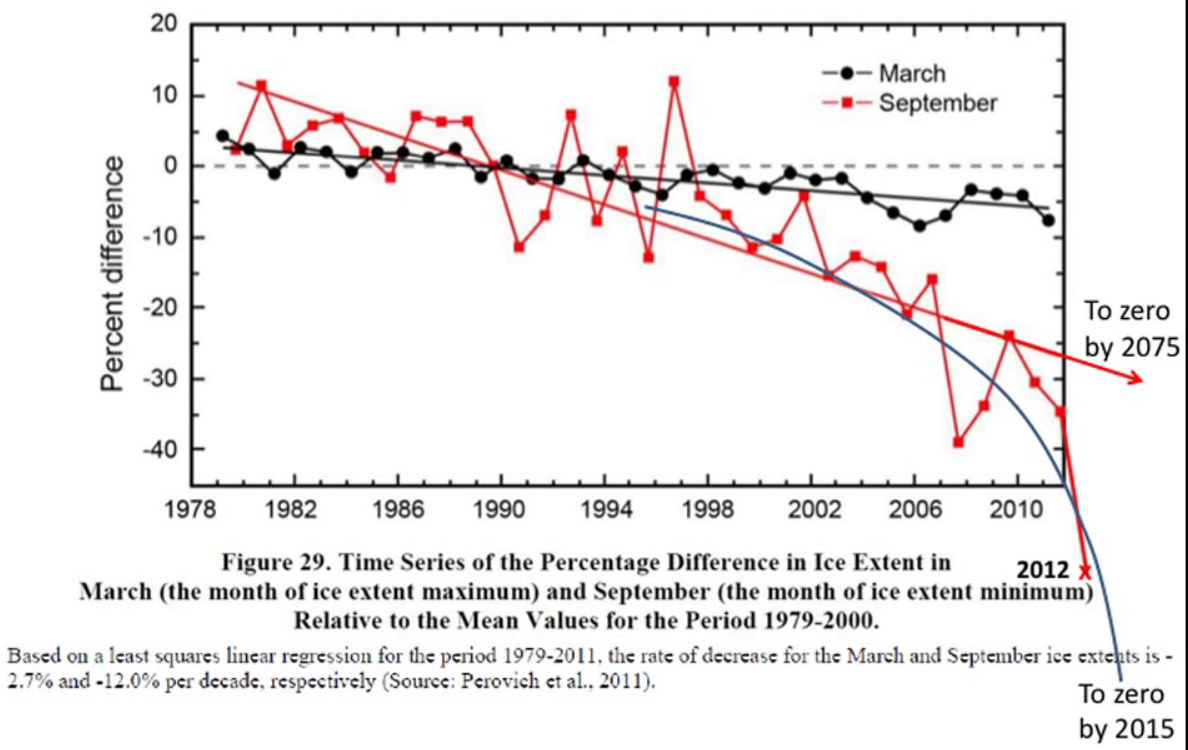
\includegraphics[width=0.8\textwidth]{arctic_feedback_dynamics_extrapolation_slide.png}
    \end{figure}

    image of you tube video frame at 11:22 minutes

    \note{extrapolation of fit "predicts" that all ice will
    disappear in the northern summer of 2015}

\end{frame}

\begin{frame}

    image of arctic sea ice extent in summer of 2015 (third lowest since
    measurements began)

    Evidence suggests otherwise, so \ldots huh?

\end{frame}

\begin{frame}

    background info

    the talk is from 2013, using data from 2012 (are the dates correct
    here?; confirm result using program later in talk?)

    used a "curved" fit of the data and extrapolated from that to conjecture
    that in roughly 2015 the arctic sea ice would disappear in summer

    not clear what kind of fit is shown

    the point David Wasdell makes, is that one can't use a linear
    interpolation as the basis of recommendations for decision makers

    so maybe it looked that bad back then

\end{frame}

\begin{frame}

    the arctic sea ice extent data are freely available online (back to the
    70's), so we can check the analysis and maybe reproduce the result

    with up to date data we can also make our own "prediction"

    link to NSIDC

    NSIDC logo

\end{frame}

\begin{frame}
sea ice extent data is available for free online, back to the 70's (NSIDC).  I can
run the investigation similarly myself...
\end{frame}

first quick look at data with a spreadsheet, however that's not fun, and I
want to be able to run the program more often and maybe fiddle with things a
bit more than I can with a spreadsheet.  So, I pulled out my favourite swiss
army chainsaw.

- grab data (LWP::Simple)
- hey, it's CSV (Text::CSV)
- comes in two files, "archive" and "near real time (nrt)"
- stitch them together
- extract minima for a given year
- plot minima (Gnuplot bindings???, maybe SVG::Plot???)
- fit library?  Linear regression from scratch?  (Algorithm::CurveFit)
- what is the equation for the the fit?  (Python module, since there isn't a
Perl module)
- high school maths -> solve for y=0
- can one reproduce the old result from the video?
- what does the extrapolation tell us?
- mention technologies/modules used

\begin{frame}
linear is obviously wrong
exponential doesn't give as good a fit as 2nd order polynomial
\end{frame}

\begin{frame}
    \frametitle{Think!}
    \begin{itemize}
	\item Don't believe everything you read in blogs
	\item Don't believe every video you see online
	\item FFS don't believe me!
	\item Critically evalutate everything
	\item The tools are in \emph{your} hands, the data is available for
	    free, can come to own conclusion.
	    \begin{itemize}
		\item Perl, CPAN, freely available data, your brain
	    \end{itemize}
    \end{itemize}
\end{frame}




% - working for DNPS
% - did not only development, but also ran social media stuff
% - in Twitter feed came across video about Arctic feedback dynamics
% - video interesting and informative, however ...
% - makes a prognosis about Arctic sea ice disappear in summer 2015
% - uses data up to 2011 and sort of 2012, was uploaded on 2013, I saw the
%   video in 2014 and, well, it's taken longer to prepare this talk than I
%   would have liked
% - Arctic sea ice wasn't gone in the northern summer of 2015, so... wtf?
% - wtf is how one writes hä in English
% - the data is freely available online (e.g. NSIDC), so why not check the
%   results? (btw, verification of results is an important part of science)
% - let's look at the presented results carefully: a linear fit of the
%   1979-2011 data gives a zero crossing in 2075; "using the curves" and
%   data from what looks like 1995-2012 (data point at 2012 looks too low),
%   gives a zero crossing at 2015
% - where do I get the data?
% - it's in an archived form, and as near-real-time
% - stich them together, plot
% - we really want the minima, extract them
% - what's the linear fit?
% - what's the zero crossing of the linear fit?  (roughly 2073, so given
%   errors a verification of result presented in talk)
% - talk uses a fit-data-and-extrapolate approach; we can do that too
% - a second order polynomial fits quite well


% - take away message: don't believe everything!  Think critically!  Use
%   your brain and the tools at hand.  The tools and data are often freely
%   available.

\end{document}
